% chktex-file 8

\providecommand{\keywords}[1]{\textbf{\textit{Index terms---}} #1}

\newcommand{\abs}[1]{ \left\lvert#1\right\rvert}
\newcommand{\norm}[1]{\left\lVert#1\right\rVert}

\newcommand{\embed}{\text{embed}}
\newcommand{\f}{\text{f}}
\newcommand{\itc}{\text{itc}}
\newcommand{\mfd}{\text{mfd}}
\newcommand{\nn}{\text{nn}}

\newcommand{\E}{\mathrm{E}}

\newcommand{\Latap}{\mathcal{L}_\mathrm{atap}}
\newcommand{\Latrl}{\mathcal{L}_\mathrm{atrl}}
\newcommand{\Lcerl}{\mathcal{L}_\mathrm{cerl}}
\newcommand{\Lfmrl}{\mathcal{L}_\mathrm{fmrl}}

\newcommand{\adamSingleFigure}[3]{%
  \begin{figure}
    \centering
    \includegraphics[width=\columnwidth]{#1}%
    \caption{#3}%
    \label{#2}
  \end{figure}
}

\newcommand{\adamSingleFigureCS}[4]{%
  \begin{figure}
    \centering
    \includegraphics[width=#1\columnwidth]{#2}%
    \caption{#4}%
    \label{#3}
  \end{figure}
}

\newcommand{\adamIncludeFigure}[3]{
  \subcaptionbox{#2}{\includegraphics[width=#1\columnwidth]{#3}}
}

\newcommand{\adamIncludeFigureNC}[2]{
  \includegraphics[width=#1\columnwidth]{#2}
}

\newcommand{\adamIncludeFigureCS}[4]{
  \subcaptionbox{#3}[#2\columnwidth]{\includegraphics[width=#1\columnwidth]{#4}}
}

\newcommand{\figureVarVapComparison}{
  % fig:var_vap_comparison
  \noindent
  \begin{figure}
    \centering
    \captionsetup[sub]{labelformat=empty}
    \begin{tabular}{ccccccccc}
      \adamIncludeFigureNC{0.08}{images/VariancePoolingImpact/var-000000.png}
      \adamIncludeFigureNC{0.08}{images/VariancePoolingImpact/var-005000.png}
      \adamIncludeFigureNC{0.08}{images/VariancePoolingImpact/var-010000.png}
      \adamIncludeFigureNC{0.08}{images/VariancePoolingImpact/var-015000.png}
      \adamIncludeFigureNC{0.08}{images/VariancePoolingImpact/var-020000.png}
      \adamIncludeFigureNC{0.08}{images/VariancePoolingImpact/var-025000.png}
      \adamIncludeFigureNC{0.08}{images/VariancePoolingImpact/var-030000.png}
      \adamIncludeFigureNC{0.08}{images/VariancePoolingImpact/var-035000.png}
      \adamIncludeFigureNC{0.08}{images/VariancePoolingImpact/var-040000.png}
      \\
      \adamIncludeFigureNC{0.08}{images/VariancePoolingImpact/vap-000000.png}
      \adamIncludeFigureNC{0.08}{images/VariancePoolingImpact/vap-005000.png}
      \adamIncludeFigureNC{0.08}{images/VariancePoolingImpact/vap-010000.png}
      \adamIncludeFigureNC{0.08}{images/VariancePoolingImpact/vap-015000.png}
      \adamIncludeFigureNC{0.08}{images/VariancePoolingImpact/vap-020000.png}
      \adamIncludeFigureNC{0.08}{images/VariancePoolingImpact/vap-025000.png}
      \adamIncludeFigureNC{0.08}{images/VariancePoolingImpact/vap-030000.png}
      \adamIncludeFigureNC{0.08}{images/VariancePoolingImpact/vap-035000.png}
      \adamIncludeFigureNC{0.08}{images/VariancePoolingImpact/vap-040000.png}
    \end{tabular}
    \caption{The gradient impact comparison between variance and variance pooling during training. The first row shows the impact of variance while the second shows that of variance pooling. The visualization interval is 5000 steps of gradient backpropagation on the corresponding image.}%
    \label{fig:var_vap_comparison}
  \end{figure}
}

\newcommand{\figureEmbeddingExtractionArchitecture}{
  % fig:embedding_extraction_architecture
  \begin{figure}
    \centering
    \begin{tabular}{cc}
      \adamIncludeFigure{0.45}{Embedding}{images/Architecture/Architecture-Embedding.png}
      \adamIncludeFigure{0.45}{Extraction}{images/Architecture/Architecture-Extraction.png}
    \end{tabular}
    \caption{The Embedding and Extraction Architecture}%
    \label{fig:embedding_extraction_architecture}
  \end{figure}
}

\newcommand{\figureTwoModelArchitectures}{
  % fig:two_model_architectures
  \begin{figure}
    \centering
    \begin{tabular}{cc}
      \adamIncludeFigureCS{0.3}{0.4}{ITC Attention Model}{images/ITC/ITC-Model.png}
      \adamIncludeFigureCS{0.5}{0.5}{MFD Attention Model}{images/MFD/MFD-Model-Detailed-2.png}
    \end{tabular}
    \caption{Model Architectures}%
    \label{fig:two_model_architectures}
  \end{figure}
}

\newcommand{\figureItcAttentionEffect}{
  % fig:itc_attention_effect
  \begin{figure}
    \centering
    \begin{tabular}{ccc}
      \adamIncludeFigureCS{0.15}{0.25}{Original Image}{images/ImageSmoother/cover-00000000-0002.png}
      \adamIncludeFigureCS{0.15}{0.25}{ITC Attention}{images/ITC/valid-attens-0000-0000-02.png}
      \adamIncludeFigureCS{0.15}{0.25}{Weighted Image}{images/ITC/valid-smthed-0000-0000-02.png}
      \\~\\
      \adamIncludeFigureCS{0.15}{0.25}{Original Image}{images/ImageSmoother/cover-00000000-0023.png}
      \adamIncludeFigureCS{0.15}{0.25}{ITC Attention}{images/ITC/valid-attens-0000-0000-23.png}
      \adamIncludeFigureCS{0.15}{0.25}{Weighted Image}{images/ITC/valid-smthed-0000-0000-23.png}
    \end{tabular}
    \caption{The Effect of ITC Attention on Texture Complexity Reduction}%
    \label{fig:itc_attention_effect}
  \end{figure}
}

\newcommand{\figureItcAttentionFinetune}{
  % fig:itc_attention_finetune
  \begin{figure}
    \centering
    \begin{tabular}{cccc}
      \adamIncludeFigure{0.15}{}{images/ImageSmoother/cover-00000000-0002.png}
      \adamIncludeFigure{0.15}{}{images/ITC/valid-attens-0000-0000-02.png}
      \adamIncludeFigure{0.15}{}{images/Finetune/min/cover-vm-attn-0000-0002.png}
      \adamIncludeFigure{0.15}{}{images/Finetune/mean/cover-vm-attn-0000-0002.png}
      \\~\\
      \adamIncludeFigure{0.15}{}{images/ImageSmoother/cover-00000000-0023.png}
      \adamIncludeFigure{0.15}{}{images/ITC/valid-attens-0000-0000-23.png}
      \adamIncludeFigure{0.15}{}{images/Finetune/min/cover-vm-attn-0000-0023.png}
      \adamIncludeFigure{0.15}{}{images/Finetune/mean/cover-vm-attn-0000-0023.png}
    \end{tabular}
    \caption{ITC Attention After Finetune}%
    \label{fig:itc_attention_finetune}
    \vspace{\baselineskip}
    The first column shows the original image, the second column shows the ITC attention before any finetune, the third column shows the ITC attention after finetuning for minima fusion strategy, and the forth column shows the ITC attention after finetuning for mean fusion strategy.
  \end{figure}
}

\newcommand{\figureMfdAttentionEffect}{
  % fig:mfd_attention_effect
  \begin{figure}
    \centering
    \begin{tabular}{ccc}
      \adamIncludeFigureCS{0.15}{0.3}{The Cover}{images/ImageSmoother/cover-00000000-0002.png}
      \adamIncludeFigureCS{0.15}{0.3}{MFD Attention}{images/MFD/valid-cover-attn-0000-0002.png}
      \adamIncludeFigureCS{0.15}{0.3}{The Embedded}{images/MFD/valid-stego-0000-0002.png}
      \\~\\
      \adamIncludeFigureCS{0.15}{0.3}{The Cover}{images/ImageSmoother/cover-00000000-0023.png}
      \adamIncludeFigureCS{0.15}{0.3}{MFD Attention}{images/MFD/valid-cover-attn-0000-0023.png}
      \adamIncludeFigureCS{0.15}{0.3}{The Embedded}{images/MFD/valid-stego-0000-0023.png}
    \end{tabular}
    \caption{The Visual Effect of MFD Attention on Embedding with Random Noise}%
    \label{fig:mfd_attention_effect}
  \end{figure}
}

\newcommand{\figureMfdEncoderDecoderBlock}{
  % fig:mfd_encoder_decoder_block
  \begin{figure}
    \centering
    \begin{tabular}{cc}
      \adamIncludeFigure{0.35}{Encoder}{images/MFD/MFD-Model-Encoder-Block.png}
      \adamIncludeFigure{0.35}{Decoder}{images/MFD/MFD-Model-Decoder-Block.png}
    \end{tabular}
    \caption{The Encoder and Decoder Block of the MFD Attention Model}%
    \label{fig:mfd_encoder_decoder_block}
  \end{figure}
}

\newcommand{\figureImageSmoothingComparison}{
  % fig:image_smoothing_comparison
  \begin{figure}
    \centering
    \begin{tabular}{cccc}
      \adamIncludeFigureCS{0.15}{0.2}{Original}{images/ImageSmoother/cover-00000000-0002.png}
      \adamIncludeFigureCS{0.15}{0.2}{Average} {images/ImageSmoother/0000-average-0002.png}
      \adamIncludeFigureCS{0.15}{0.2}{Gaussian}{images/ImageSmoother/0000-gaussian-0002.png}
      \adamIncludeFigureCS{0.15}{0.2}{Median}  {images/ImageSmoother/0000-median-0002.png}
      \\~\\
      \adamIncludeFigureCS{0.15}{0.2}{Original}{images/ImageSmoother/cover-00000000-0023.png}
      \adamIncludeFigureCS{0.15}{0.2}{Average} {images/ImageSmoother/0000-average-0023.png}
      \adamIncludeFigureCS{0.15}{0.2}{Gaussian}{images/ImageSmoother/0000-gaussian-0023.png}
      \adamIncludeFigureCS{0.15}{0.2}{Median}  {images/ImageSmoother/0000-median-0023.png}
    \end{tabular}
    \caption{Image Smoothing Effect Comparison}%
    \label{fig:image_smoothing_comparison}
  \end{figure}
}

\newcommand{\figureSteganographyResultMeanLSMOne}{
  % fig:steganography_result_mean_lsm_1
  \begin{figure}
    \centering
    \begin{tabular}{ccc}
      \adamIncludeFigureCS{0.15}{0.3}{The Cover}      {images/Inference/mean-ILSBN1/cover-00000000-0002.png}
      \adamIncludeFigureCS{0.15}{0.3}{Fused Attention}{images/Inference/mean-ILSBN1/cover-fusion-attention-00000000-0002.png}
      \adamIncludeFigureCS{0.15}{0.3}{The Embedded}   {images/Inference/mean-ILSBN1/stego-00000000-0002.png}
      \\~\\
      \adamIncludeFigureCS{0.15}{0.3}{The Cover}      {images/Inference/mean-ILSBN1/cover-00000000-0023.png}
      \adamIncludeFigureCS{0.15}{0.3}{Fused Attention}{images/Inference/mean-ILSBN1/cover-fusion-attention-00000000-0023.png}
      \adamIncludeFigureCS{0.15}{0.3}{The Embedded}   {images/Inference/mean-ILSBN1/stego-00000000-0023.png}
    \end{tabular}
    \caption{Steganography using Mean Fusion with 1-bit LSM}%
    \label{fig:steganography_result_mean_lsm_1}
  \end{figure}
}

\newcommand{\figureROCCurves}{
  % fig:roc_curves
  \begin{figure}
    \centering
    \begin{tabular}{cc}
      \adamIncludeFigure{0.48}{StegExpose}      {images/ROC-Comparison/BASN-StegExpose-Comparison-ROC.eps}%
      \adamIncludeFigure{0.48}{SPAM Features}   {images/ROC-Comparison/SPAM686-ROC.eps}%
      \\~\\
      \adamIncludeFigure{0.48}{SRM Features}    {images/ROC-Comparison/SRM-ROC.eps}
      \adamIncludeFigure{0.48}{YedroudjNet}     {images/ROC-Comparison/YedroudjNet-ROC.eps}%
    \end{tabular}
    \caption{ROC Curves: Steganalysis with StegExpose, SPAM Features, SRM Features and Yedroudj-Net}%
    \label{fig:roc_curves}
  \end{figure}
}

\newcommand{\figureBASNFeatureDistortionRate}{
  % fig:basn_feature_distortion_rate
  \adamSingleFigureCS{0.6}{%
    images/BASN-Feature-Distortion-Rate/FDR-all.eps%
  }{%
    fig:basn_feature_distortion_rate%
  }{
    ResNet-18 Classification Feature Distortion Rate
  }
}

\newcommand{\figureSoftAreaPenalty}{
  % fig:soft_area_penalty
  \begin{figure}
    \centering
    \begin{tabular}{cc}
      \adamIncludeFigure{0.3}{ITC Area Penalty}{images/ITC/ITC-Area-Penalty.eps}
      \adamIncludeFigure{0.3}{MFD Area Penalty}{images/MFD/MFD-Area-Penalty.eps}
    \end{tabular}
    \caption{Soft Area Penalties}%
    \label{fig:soft_area_penalty}
  \end{figure}
}

\newcommand{\figureFinetuneFirstPhase}{
  % fig:finetune_first_phase
  \begin{figure}
    \centering
    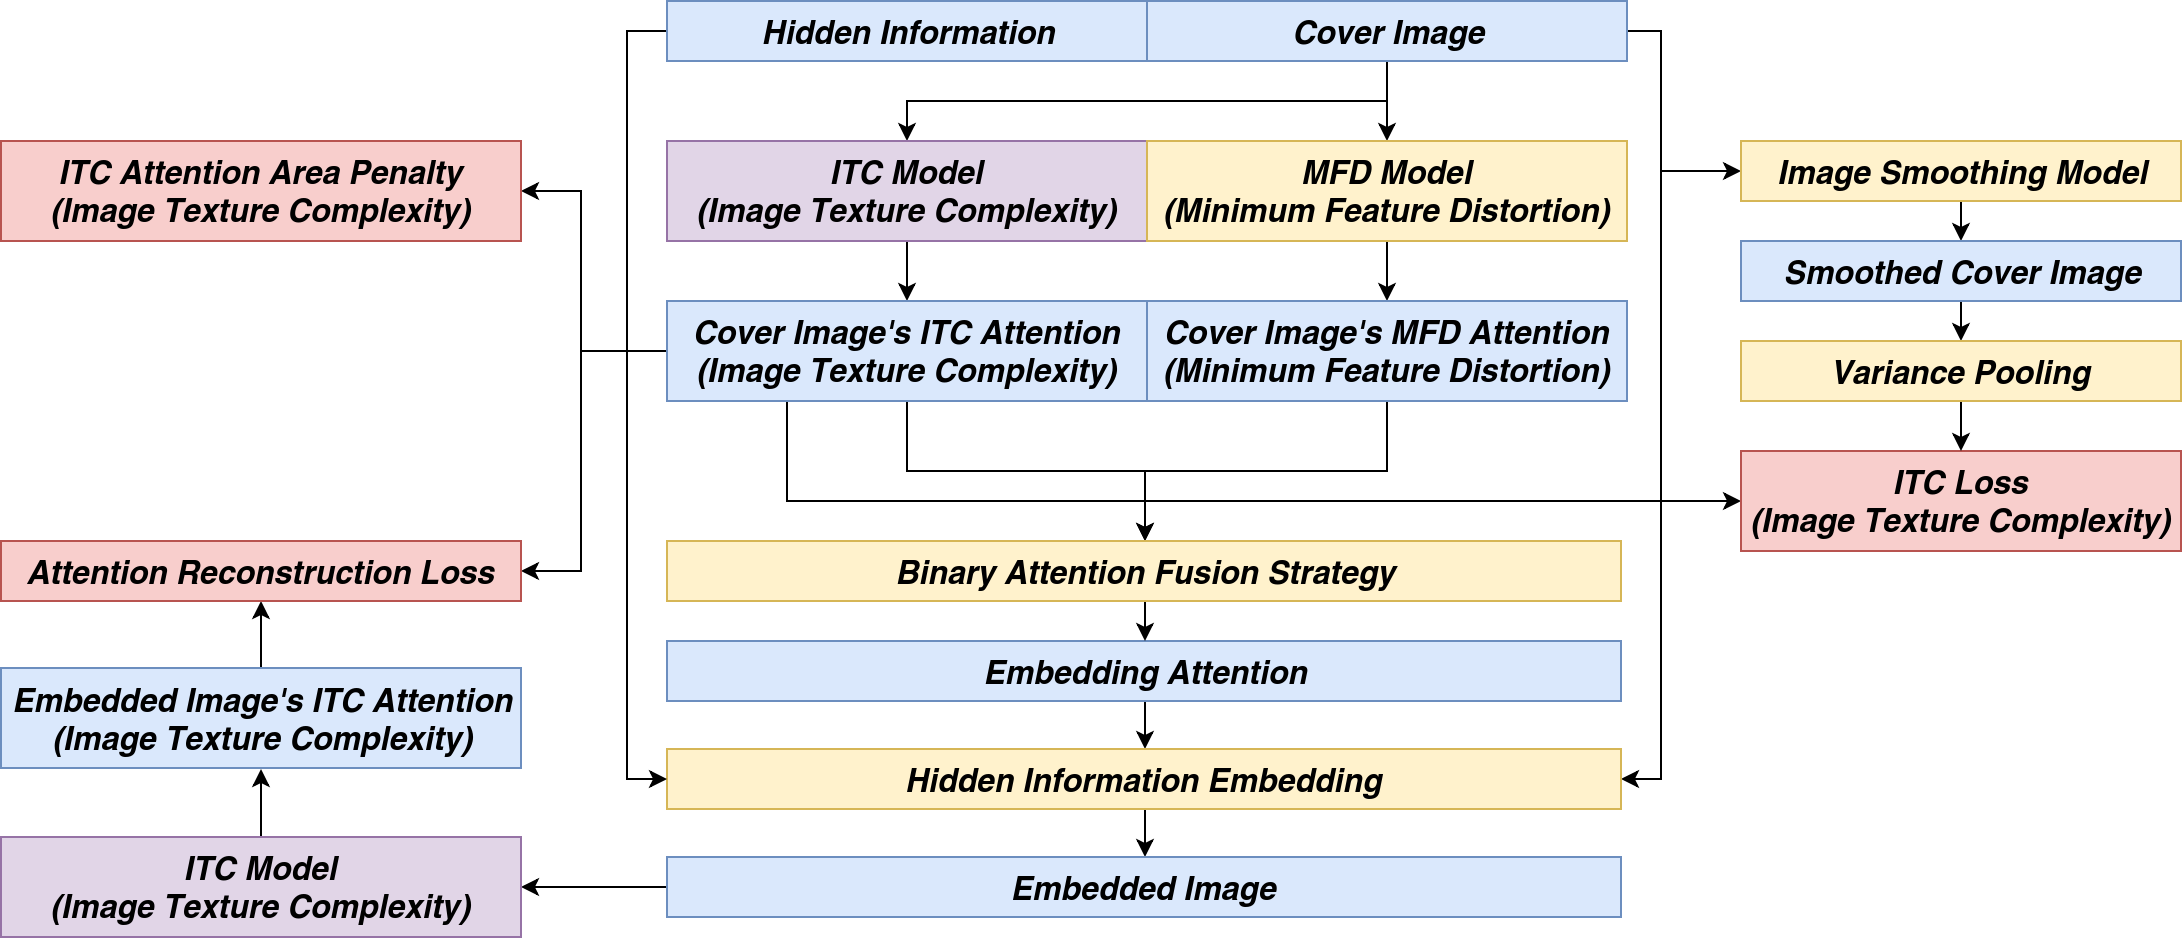
\includegraphics[width=0.9\columnwidth]{images/Finetune/Finetune-Phase-1.png}
    \caption{The \(1^{st}\) Phase Finetune Pipeline}%
    \label{fig:finetune_first_phase}
  \end{figure}
}

\newcommand{\figureMFDModelOverall}{
  % fig:mfd_model_overall
  \begin{figure}
    \centering
    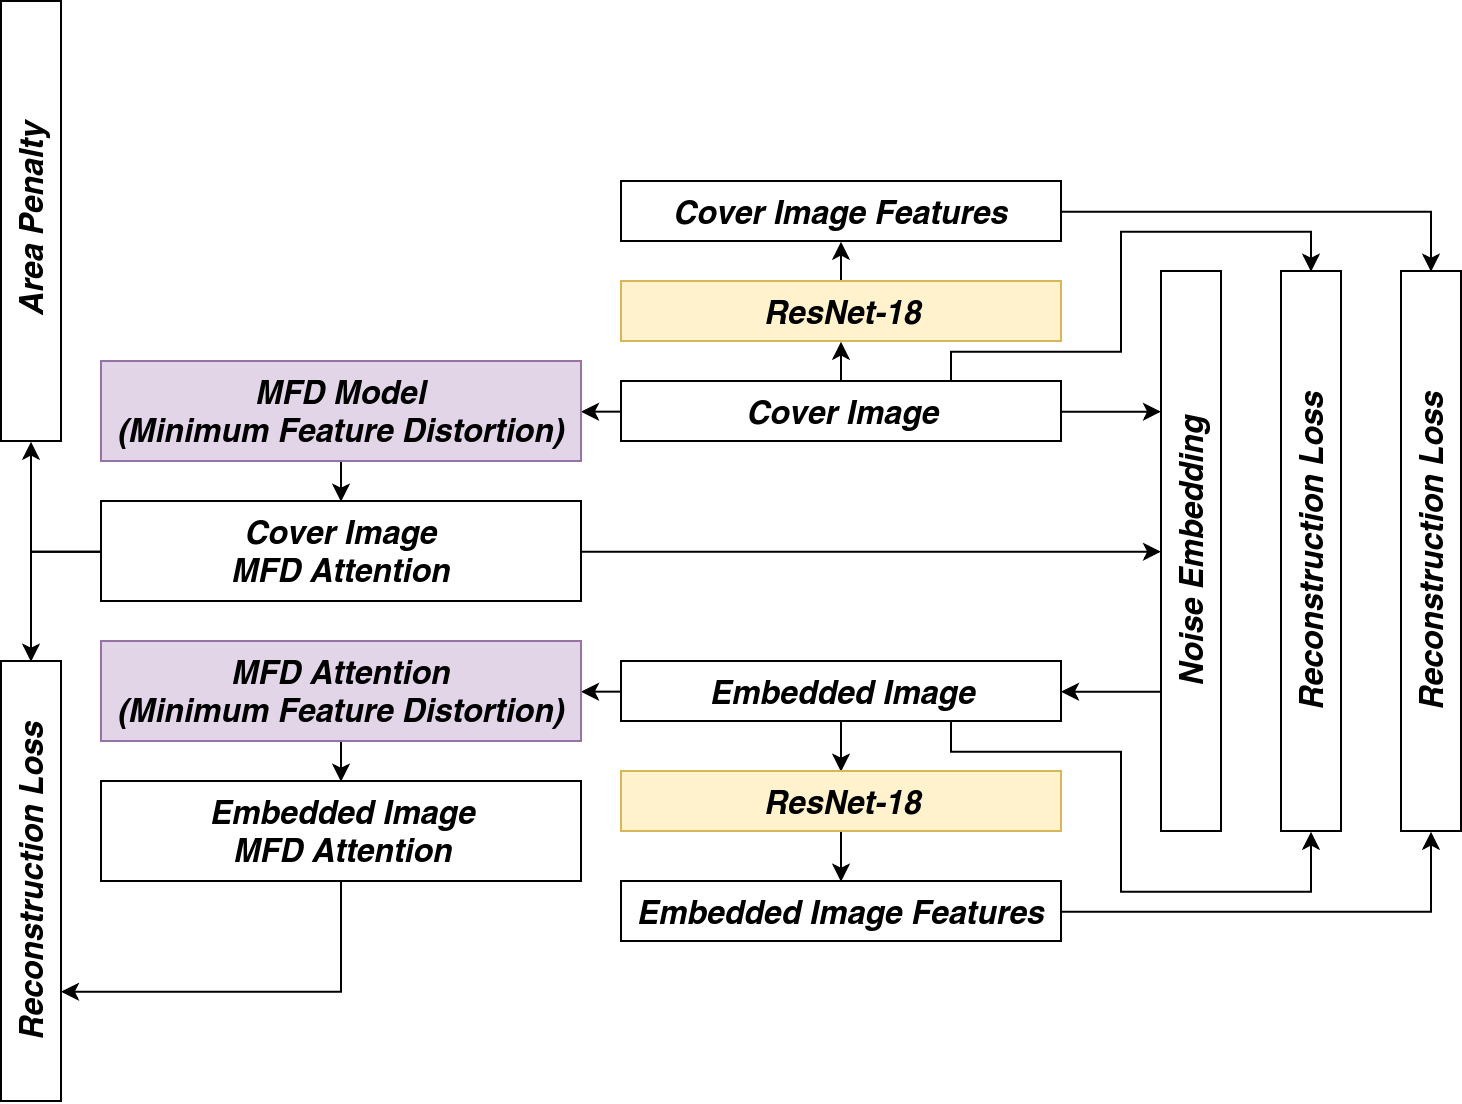
\includegraphics[width=0.8\columnwidth]{images/MFD/MFD-Model-Overall.png}
    \caption{MFD Attention Mechanism Training Pipeline}%
    \label{fig:mfd_model_overall}
  \end{figure}
}
